\documentclass{beamer}
\usetheme{Boadilla}

\usepackage{tikz}
\usetikzlibrary{shapes}

\title{Git Gud}
\author{Neil Ashford}
\institute{UQ Computing Society}
\date{2018-04-23T17:30+10:00}

\AtBeginSection[]
{
    \begin{frame}
        \frametitle{Outline}
        \tableofcontents[currentsection]
    \end{frame}
}

\begin{document}

\begin{frame}
    \titlepage
\end{frame}

\section{Introduction}

\subsection{Who am I}
\begin{frame}
    \frametitle{Who am I}
    \begin{itemize}[<+->]
        \item Neil Ashford
        \item 4th year Software\only<2->{\footnote{ish}} Engineering
        \item Committee member
        \item \texttt{@artemis} on slack, \url{ashfordneil0@gmail.com}
    \end{itemize}
\end{frame}

\subsection{What is this talk}
\begin{frame}
    \frametitle{What is this talk}
    Target Audience
    \pause
    \begin{itemize}[<+->]
        \item People who have never used version control.
        \item People who have ``memorised 5 shell commands and trust them implicitly without understanding''
    \end{itemize}
    \pause
    What I'll Cover
    \begin{itemize}[<+->]
        \item Some really basic version control you're familiar with, and its flaws.
        \item The pieces of a mental model of proper version control.
        \item How git represents each of those pieces to you.
        \item Flaws with git, and alternatives.
    \end{itemize}
\end{frame}

\section{The Version Control We Know}

\subsection{Meet the Culprit}
\begin{frame}
    \frametitle{Meet the Culprit}
    \begin{itemize}[<+->]
        \item Live demos suck, so we're trying to stick with something familiar.
        \item Please welcome our old friend...
        \item Microsoft Word\only<3->{\footnote{Okay I'm on a mac so it's pages but still}}
    \end{itemize}
\end{frame}

\subsection{Undo / Reverts}
\begin{frame}
    \frametitle{Undo / Reverts}

    \begin{columns}
        \begin{column}{0.5\textwidth}
            \begin{itemize}[<+->]
                    \pause
                \item Type ``Hello''
                \item Type ``World''
                \item Type ``Filler Text''
                \item Press Undo
                \item Press Redo
                \item Press Undo again
            \end{itemize}
        \end{column}
        \begin{column}{0.5\textwidth}
            \begin{tikzpicture}
                \only<2->{
                    \node[circle, draw, minimum size=1cm] (A) at (0,0) {Hello};
                }
                \only<3->{
                    \node[circle, draw, minimum size=1cm] (B) at (0,-2) {World};
                    \draw[->] (A) -- (B);
                }
                \only<4,6>{
                    \node[circle, draw, minimum size=1cm] (C) at (0,-4) {Filler Text};
                    \draw [->] (B) -- (C);
                }
                \only<5,7>{
                    \node[gray, dashed, circle, draw, minimum size=1cm] (C) at (0,-4) {Filler Text};
                    \draw [gray, dashed, ->] (B) -- (C);
                }
            \end{tikzpicture}
        \end{column}
    \end{columns}
\end{frame}

\subsection{Branches}
\begin{frame}
    \frametitle{Branches}

    \begin{columns}
        \begin{column}{0.5\textwidth}
            \begin{itemize}[<+->]
                \item From where we were before...
                \item Type ``Lorem Ipsum''
                \item Realise we want ``Filler Text'' back
                \item Press Undo
                \item Press Redo
                \item Weep
            \end{itemize}
        \end{column}
        \begin{column}{0.5\textwidth}
            \begin{tikzpicture}
                \only<1->{
                    \node[circle, draw, minimum size=1cm] (A) at (0,0) {Hello};
                    \node[circle, draw, minimum size=1cm] (B) at (0,-2) {World};
                    \draw[->] (A) -- (B);
                }
                \only<1>{
                    \node[gray, dashed, circle, draw, minimum size=1cm] (C) at (0,-4) {Filler Text};
                    \draw[gray, dashed, ->] (B) -- (C);
                }
                \only<2->{
                    \node[red, dashed, circle, draw, minimum size=1cm] (C) at (0,-4) {Filler Text};
                    \draw[red, dashed, ->] (B) -- (C);
                }
                \only<2,3,5->{
                    \node[circle, draw, minimum size=1cm] (D) at (3,-4) {Lorem Ipsum};
                    \draw[->] (B) -- (D);
                }
                \only<4>{
                    \node[gray, dashed, circle, draw, minimum size=1cm] (D) at (3,-4) {Lorem Ipsum};
                    \draw[gray, dashed, ->] (B) -- (D);
                }
            \end{tikzpicture}
        \end{column}
    \end{columns}
\end{frame}

\subsection{Merges and Collaborative Work}
\begin{frame}
    \frametitle{Merges and Collaborative Work}

    \begin{columns}
        \begin{column}{0.5\textwidth}
            \begin{itemize}[<+->]
                \item From where we were before...
                \item Save it, throw it on a USB, give it to a friend
                \item \textbf{We} write ``dolor sit amet'' at the \textbf{end} of the document
                \item \textbf{They} write ``git is cool'' at the \textbf{top} of the document
                \item How to combine these?
            \end{itemize}
        \end{column}
        \begin{column}{0.5\textwidth}
            \resizebox{\textwidth}{!}{
                \begin{tikzpicture}
                    \only<1->{
                        \node[circle, draw, minimum size=1cm] (A) at (0,0) {Hello};
                        \node[circle, draw, minimum size=1cm] (B) at (0,-2) {World};
                        \draw[->] (A) -- (B);
                        \node[gray, dashed, circle, draw, minimum size=1cm] (C) at (0,-4) {Filler Text};
                        \draw[gray, dashed, ->] (B) -- (C);
                        \node[circle, draw, minimum size=1cm] (D) at (3,-4) {Lorem Ipsum};
                        \draw[->] (B) -- (D);
                    }
                    \only<3->{
                        \node[blue, circle, draw, minimum size=1cm] (E) at (3,-7) {dolor sit amet};
                        \draw[blue, ->] (D) -- (E);
                    }
                    \only<4->{
                        \node[green, circle, draw, minimum size=1cm] (F) at (6,-6) {git is cool};
                        \draw[green, ->] (D) -- (F);
                    }
                    \only<5>{
                        \node[circle, draw, minimum size=1cm] (G) at (4.5, -9) {merge};
                        \draw[->] (E) -- (G);
                        \draw[->] (F) -- (G);
                    }
                \end{tikzpicture}
            }
        \end{column}
    \end{columns}
\end{frame}

\section{A Git Mental Model}

\subsection{Differences Between Our Live Demo and Git}
\begin{frame}
    \frametitle{Differences Between Our Live Demo and Git}

    \begin{columns}
        \begin{column}{0.5\textwidth}
            \begin{itemize}[<+->]
                \item Microsoft Word can't do all of these things
                \item (Git can)
                \item Undo and Redo track really small changes in a single file
                \item Git tracks larger changes, in a directory (hereafter, repository)
                \item ...and more
            \end{itemize}
        \end{column}
        \begin{column}{0.5\textwidth}
            \resizebox{\textwidth}{!}{
                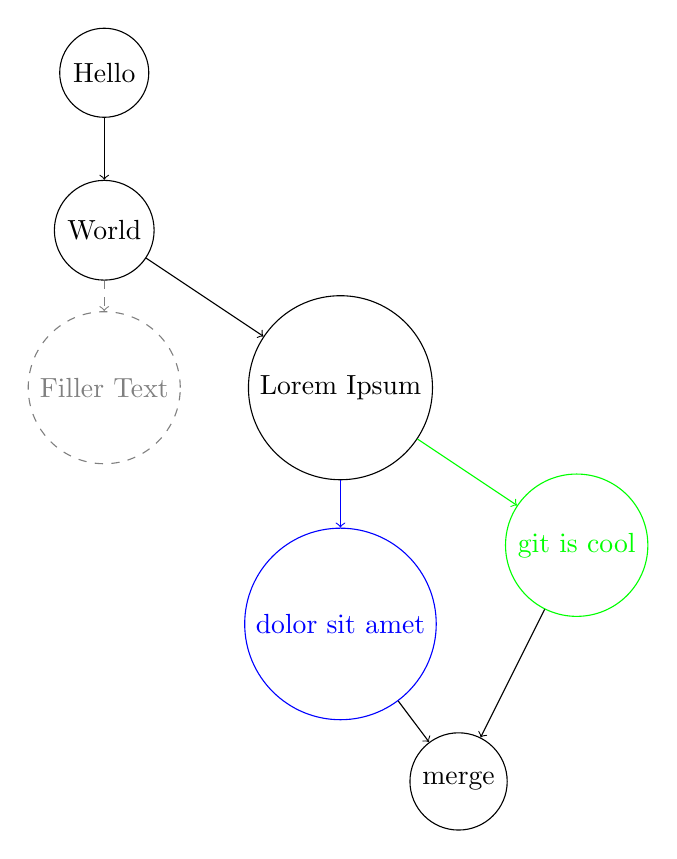
\begin{tikzpicture}
                    \node[circle, draw, minimum size=1cm] (A) at (0,0) {Hello};
                    \node[circle, draw, minimum size=1cm] (B) at (0,-2) {World};
                    \draw[->] (A) -- (B);
                    \node[gray, dashed, circle, draw, minimum size=1cm] (C) at (0,-4) {Filler Text};
                    \draw[gray, dashed, ->] (B) -- (C);
                    \node[circle, draw, minimum size=1cm] (D) at (3,-4) {Lorem Ipsum};
                    \draw[->] (B) -- (D);
                    \node[blue, circle, draw, minimum size=1cm] (E) at (3,-7) {dolor sit amet};
                    \draw[blue, ->] (D) -- (E);
                    \node[green, circle, draw, minimum size=1cm] (F) at (6,-6) {git is cool};
                    \draw[green, ->] (D) -- (F);
                    \node[circle, draw, minimum size=1cm] (G) at (4.5, -9) {merge};
                    \draw[->] (E) -- (G);
                    \draw[->] (F) -- (G);
                \end{tikzpicture}
            }
        \end{column}
    \end{columns}
\end{frame}

\subsection{Commits}
\begin{frame}
    \frametitle{Commits}

    \begin{columns}
        \begin{column}{0.5\textwidth}
            \begin{itemize}[<+->]
                \item The \textbf{atomic unit} of git
                \item You make the commits
                \item A commit consists of 3 things
                \item The state of the repo when that commit was made
                \item What commit(s) came immediately before it
                \item Metadata (timestamp, author, cryptographic hash)
            \end{itemize}
        \end{column}
        \begin{column}{0.5\textwidth}
            \begin{tikzpicture}
                \node[circle, draw, minimum size=5cm] (A) at (0,0) {Hello};
            \end{tikzpicture}
        \end{column}
    \end{columns}
\end{frame}

\end{document}
